% ncse_new/\problems/\chpt/ex_Kron.tex
% solutions require:    Kron_B.m     Kron_C.m     mainKron.m     kron_timings.eps

\renewcommand{\chpt}{ch_matvec}

\begin{problem}[Kronecker product] 
\label{prb:Kron}

In \lref{def:kron} we learned about the so-called Kronecker product, available
in \matlab{} through the command \texttt{kron}. In this problem we revisit the
discussion of \lref{ex:kron}. Please refresh yourself on this example and
study \lref{mc:kronmultv} again. 

As in \lref{ex:kron}, the starting point is the line of \matlab{} code
\begin{equation} \label{eq:ex_Kron}
  \mathbf{y}=\tt{kron(A,B)*x},
\end{equation} 
where the arguments are $\mathbf{A},\mathbf{B} \in \IR^{n,n}, \mathbf{x} \in \IR^{n \cdot n}$.

%%%%%%%%%%%% SUBPROBLEM 1

\begin{subproblem}[1] \label{subprb:Kron_1}
Obtain further information about the \texttt{kron} command from \Matlab~ help
issuing \texttt{doc kron} in the \matlab{} command window. 

\begin{solution}
See \Matlab~ help.
\end{solution}
\end{subproblem}

%%%%%%%%%%%% SUBPROBLEM 2

\begin{subproblem}[1] \label{subprb:Kron_2}
Explicitly write \cref{eq:ex_Kron}
in the form $\mathbf{y}=\mathbf{M} \mathbf{x}$ (i.e. write down $\vec{M}$), for
$\mathbf{A}=\begin{pmatrix}
         1 & 2   \\
         3 & 4   \\
 \end{pmatrix}$
and
$\mathbf{B}=\begin{pmatrix}
         5 & 6   \\
         7 & 8   \\
 \end{pmatrix}$.

\begin{solution}
$\Vy=\begin{pmatrix}
         5 & 6 & 10 & 12  \\
         7 & 8 & 14 & 16  \\
         15 & 18 & 20 & 24  \\
         21 & 24 & 28 & 32  \\
 \end{pmatrix}\Vx$.
\end{solution}
\end{subproblem}

%%%%%%%%%%%% SUBPROBLEM 3

\begin{subproblem}[1] \label{subprb:Kron_3}
What is the asymptotic complexity ($\to$ \lref{def:comp}) 
of the \Matlab~ code \eqref{eq:ex_Kron}? Use the Landau symbol
from \lref{def:O} to state your answer. 

\begin{solution}
\texttt{kron(A,B)} results in a matrix of size $n^2 \times n^2$ and $x$ has length $n^2$. So the complexity is the same as a matrix-vector multiplication for the resulting sizes. In total this is $O(n^2*n^2)=O(n^4)$.
\end{solution}
\end{subproblem}

%%%%%%%%%%%% SUBPROBLEM 4

\begin{subproblem}[2] \label{subprb:Kron_4} Measure the runtime of
  \eqref{eq:ex_Kron} for $n=2^{3,4,5,6}$ and random matrices. Use the \matlab{} functions
  \texttt{tic} and \texttt{toc} as explained in example \ncseex{ex:effmatmult} of
  the Lecture Slides.
  
 \begin{solution}
Since \texttt{kron(A,B)} creates a large matrix consisting of smaller blocks with size $n$, i.e. $B$ multiplied with $A(i,j)$, we can split the problem up in $n$ matrix-vector multiplications of size $n$. This results in a routine with complexity $n*O(n^2)=O(n^3)$ 
The implementation is listed in \ref{mc:Kron_B}.
The runtimes are shown in Figure~\ref{fig:kron_timings}.

\lstinputlisting[caption={An efficient implementation for \ref{prb:Kron}},label={mc:Kron_B}]
{\problems/\chpt/MATLAB/Kron_B.m}
 \end{solution}

\end{subproblem}

%%%%%%%%%%%% SUBPROBLEM 5

\begin{subproblem}[2] \label{subprb:Kron_5}
  Explain in detail, why \eqref{eq:ex_Kron} can be replaced with the single line
  of \matlab{} code
  \begin{gather}
    \label{eq:Kron:sl}
    \text{\texttt{y = reshape( B * reshape(x,n,n) * A', n*n, 1); }}
  \end{gather}
  and compare the execution times of \eqref{eq:ex_Kron} and \eqref{eq:Kron:sl} for
  random matrices of size $n=2^{3,4,5,6}$.
  
\begin{solution}
\lstinputlisting[caption={A second efficient implementation for \ref{prb:Kron} using \texttt{reshape}.},label={mc:Kron_C}]
{\problems/\chpt/MATLAB/Kron_C.m}
\lstinputlisting[caption={Main routine for runtime measurements of \ref{prb:Kron}},label={mc:mainKron}]
{\problems/\chpt/MATLAB/mainKron.m}

% \begin{figure}[htb]
% \centering
% 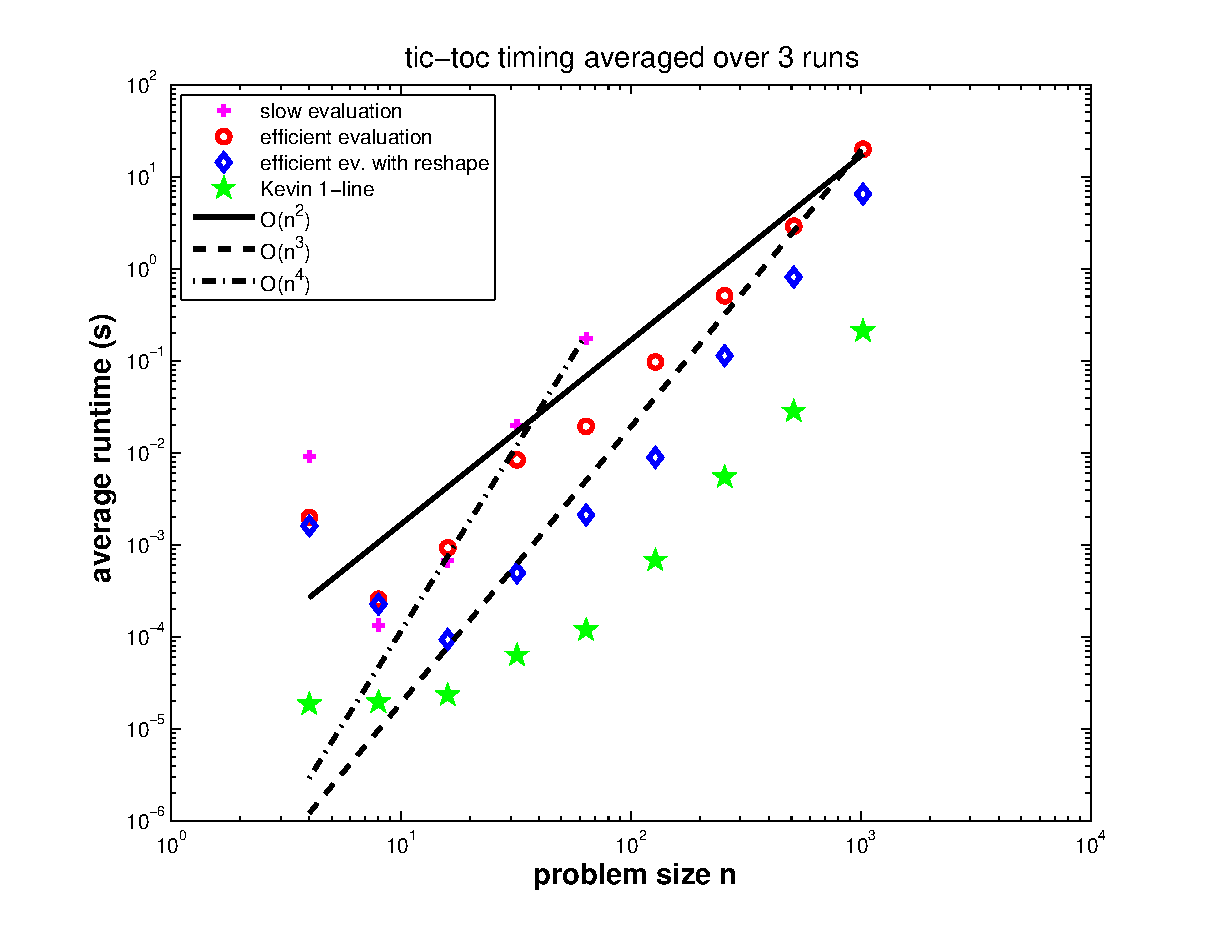
\includegraphics[width=0.8\textwidth]{\problems/\chpt/PICTURES/kron_timings.eps}
% \caption{Timings for \ref{prb:Kron}}\label{fig:kron_timings}
% \end{figure}
\end{solution}
\end{subproblem}

\begin{subproblem}[2] \label{subprb:Kron_6}
  Based on the \eigen{} numerical library ($\to$ \lref{sec:eigen}) implement a
  \Cpp{} function 
\begin{lstlisting}[style=cppsimple]
template <class Matrix>
void kron(const Matrix & A, const Matrix & B, Matrix & C) {
  // Your code here
}
\end{lstlisting}
returns the Kronecker product of the argument matrices \texttt{A} and \texttt{B}
in the matrix \texttt{C}. 

\begin{hint}
  Feel free (but not forced) to use the partial codes provided in \verb|kron.cpp| as well as the CMake file \verb|CMakeLists.txt| (including \verb|cmake-modules|) and the timing header file \verb|timer.h|~.
\end{hint}

\begin{solution}
    See \texttt{kron.cpp} or \cref{cppc:mainKron}.
\end{solution}
\end{subproblem}

\begin{subproblem}[2] \label{subprb:Kron_7}
  Devise an implementation of the \matlab{} code \eqref{eq:ex_Kron} in \Cpp according
  to the function definition
  \begin{lstlisting}[style=cppsimple]
template <class Matrix, class Vector>
void kron_mv(const Matrix & A, const Matrix & B, const Vector & x, Vector & y);
  \end{lstlisting}
  The meaning of the arguments should be self-explanatory. 

  \begin{solution}
    See \texttt{kron.cpp} or \cref{cppc:mainKron}.
  \end{solution}
\end{subproblem}

\begin{subproblem}[3] \label{subprb:kron:8}
  Now, using a function definition similar to that of the previous sub-problem,
  implement the \Cpp{} equivalent of \eqref{eq:Kron:sl} in the function
  \texttt{kron\_mv\_fast}. 

  \begin{hint}
    Study \lref{rem:eigrs} about ``reshaping'' matrices in \eigen{}.
  \end{hint}
\end{subproblem}

\begin{subproblem}[3] \label{subprb:kron:9}
  Compare the runtimes of your two implementations as you did for the \matlab{}
  implementations in sub-problem \ref{subprb:Kron_5}. 

\begin{solution}
\lstinputlisting[style=cpp,caption={Main routine for runtime measurements of \ref{prb:Kron}},label={cppc:mainKron}]
{\problems/\chpt/CPP/kron.cpp}

\begin{figure}[htb]
\centering
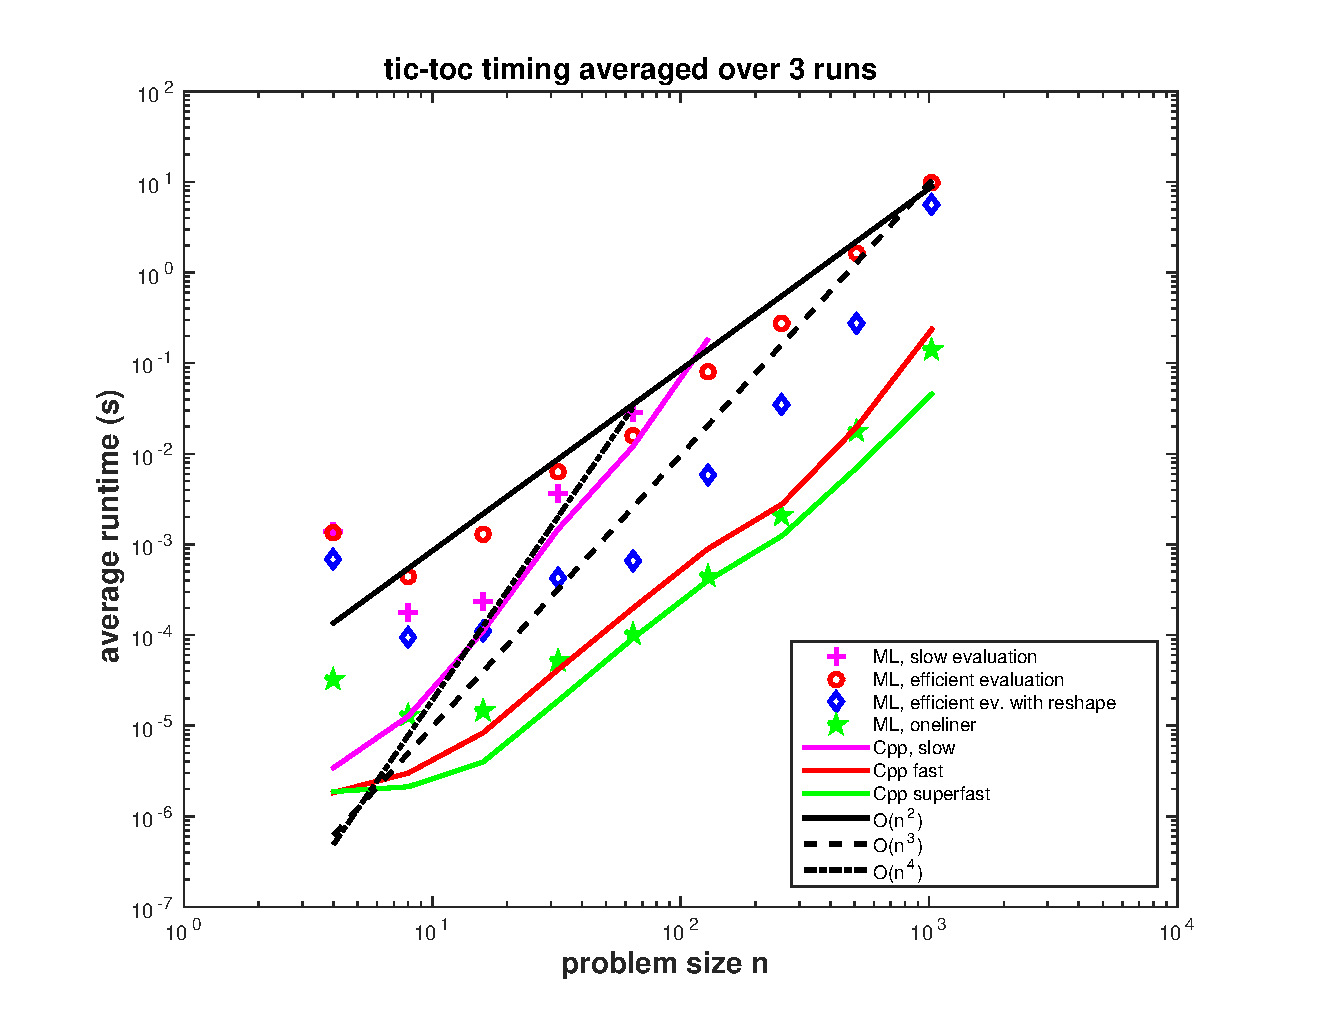
\includegraphics[width=0.8\textwidth]{\problems/\chpt/PICTURES/kron_timings_cpp.eps}
\caption{Timings for \ref{prb:Kron} with \Matlab and \Cpp implementations.} \label{fig:kron_timings}
\end{figure}
\end{solution}

\end{subproblem}

\end{problem}